\subsubsection{Recirculation algorithm}
\label{sec:models-recirc} 

The \emph{Recirculation algorithm} designed by~\citet{hinton1988learning} is an unsupervised neural letwork for learning encoder tasks. Motivation for such a model comes from interesting hidden representations of backpropagation~(\ref{sec:models-bp}) which could be used as an encoder. It has only two layers denoted \emph{visible layer} and \emph{hidden layer} as shown in Figure~\ref{fig:models-recirc}. The aim of the network is to remember on the hidden layer the patterns presented to the visible layer. This could be used for compression if the hidden layer has fewer units than the visible layer. It also could be used as a content-addressable memory, when if novel patterns are presented to the network then it could show the blend of the most similar stored patterns. 

\begin{figure}[H]
  \centering
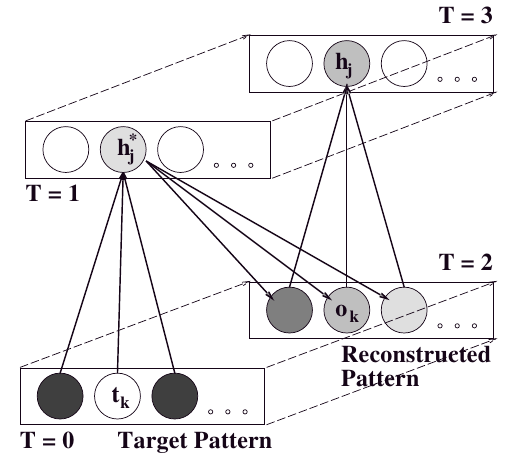
\includegraphics[width=0.4\textwidth]{img/recirculation.png}
  \caption{The recirculation algorithm by~\citet{hinton1988learning}. Taken from \citep{o1996bio}.}
  \label{fig:models-recirc}
\end{figure}

As depicted in Figure~\ref{fig:models-recirc} the activation is propagated in four steps $T \in \{0,1,2,3\}$. At the first phase, denoted by $T=0$ only the input vector $t$ is clamped on the visible layer, at $T=1$ a forward pass $h^{*}$ is computed from visible to hidden, at $T=2$ a \emph{reconstructed} pattern $o_k$ as a function of hidden state $h^{*}$ is computed and finally at $T=3$ a hidden state $h$ is computed from $o_k$.

For the reconstruction to work \emph{symmetric} weights are used. The learning rule is common for both visible and hidden layers and it's based only on the difference of activations: 
\begin{align}
\frac{\partial E}{\partial w_{ij}} &= -(\eta^{*}_j - \eta_j) \phi'(\eta_j) t_i, \nonumber \\
&\approx -(h^{*}_j - h_j)t_i. \nonumber 
\end{align} 
And similary we get $h_i(t_j - o_j)$ for the hidde to visible weights. The approximation step is possible because $\phi'(\eta_j)$ has \emph{usually} the same sign as $(\eta^{*}_j - \eta_j) $~\citep{hinton1988learning, o1996bio}. The approximation more precise if the difference of activations is smaller and therefore, the rule~(\ref{eq:models-recirc-rule}) could be used to make $o$ similar to target pattern $t$.
\begin{equation}
\label{eq:models-recirc-rule}
o_k = \alpha t_k + (1-\alpha)f(\eta_k). 
\end{equation} 

